
% !TeX root = ../main.tex
% Add the above to each chapter to make compiling the PDF easier in some editors.
\chapter{Related Work}\label{chapter:related_wrok}
This chapter provides an overview of some of the most relevant works on \acrfull{ap}. As it has been also mentioned in chapter \ref{chapter:introduction}, there are two main steps in \acrshort{ap}: 1- parking vacancy detection and 2- path/motion generation for parking maneuver. Related works in each field have been explained here.
\section{Parking Detection}
Detection of parking slot could be based on sensors or visual aspects. As it has been explained before, parking detection methods are in 2 categories: 1- free space-based approaches and 2- parking slot marking-based approaches. There is always this criticism about sensor-based methods that they depend on adjacent vehicles to find a parking vacancy and parking place which detected in this way is always surrounded by exactly two vehicles so when there is no car in front of one vehicle and still there is enough place for parking, this parking bay could not be detected \cite{visual-parking-slot}. However, the second method(visual method based on line marker) is not also perfect because it could be only applicable during day time or when there are enough lights to extract the features, photos from the parking environment should have a great quality to make it possible for classifier to find the features \cite{Laser-radar-based}. Here refers to some of the recent works in both approaches.
\subsection{Free Space-Based or Sensor-Based}
In sensor based parking vacancy detection we could point out this recent work \cite{radar-parkingDetection} based on Radar sensor as they used radar sensor for detection in all kinds of parking (parallel and perpendicular parking lots). They presented some sorts of filtering calculation and classification of parking spaces in order to optimize Radar results as they claim on 95 percent of accuracy in detected parking lots with an inexpensive algorithm. \cite{UltraSonic} used UltraSonic sensors in parking occupancy detection and they claim that their method provides accurate measurements from sides of the parking with simple calculation. In \cite{detection-ultraSonic} UltraSonic sensors have been used both in parking detection and parking maneuver. In \cite{lidar-Germany} from Hanover university of Germany, a novel idea of using Lidar sensor as a new sensor for parking occupancy detection has been presented. They believe that modern sensors provide better facility for detection and data collection and also using Lidar would help to make a more detailed and precise measurements. \cite{Laser-radar-based} presents a method to find free parking space between vehicles by scanning laser-radar. They believe that UltraSonic sensors have been successful to find parking vacancy in parallel parking but could not be used in perpendicular(or vertical) parking because of the fact that UltraSonics could work in a situation that incident angle between UltraSonic sensor and sides of adjacent vehicle is small and as this angle in perpendicular parking situation is so large, range recognition usually fails. The method that \cite{Laser-radar-based} used for parking space detection is based on corner detection. Target parking position is found based on the corner detection of parking spaces and corners are divided to round and rectangular. Finally,\cite{fixed-mobile-sensors} compares different sensor approaches and tests detection results in fixed and mobile sensor systems. Fixed approach, installs sensors in parking bays. Mobile approach is when the sensor mounted on the vehicle and gathers data as the car is moving. It has been said that mobile approach provides less accuracy but in \cite{fixed-mobile-sensors} the focus is to present a novel idea to increase accuracy. They used Sonar-sensors for mobile detection and it was working in small sensor ranges. They have also mentioned that Mobile sensors would be more expensive than fixed sensors.
\subsection{Marking-Based or Vision-Based}
As one of the best vision-based approach, we could refer to \cite{markingPointConf} where they proposed a detection method based on marking points in parking lot. Marking points are edges of the parking places which are the conjunction of line markers that separates parking place for each vehicle as it can be seen in fig \ref{fig:markingPoint}.
\begin{figure}
\centering
    \begin{tabular}{lc}
         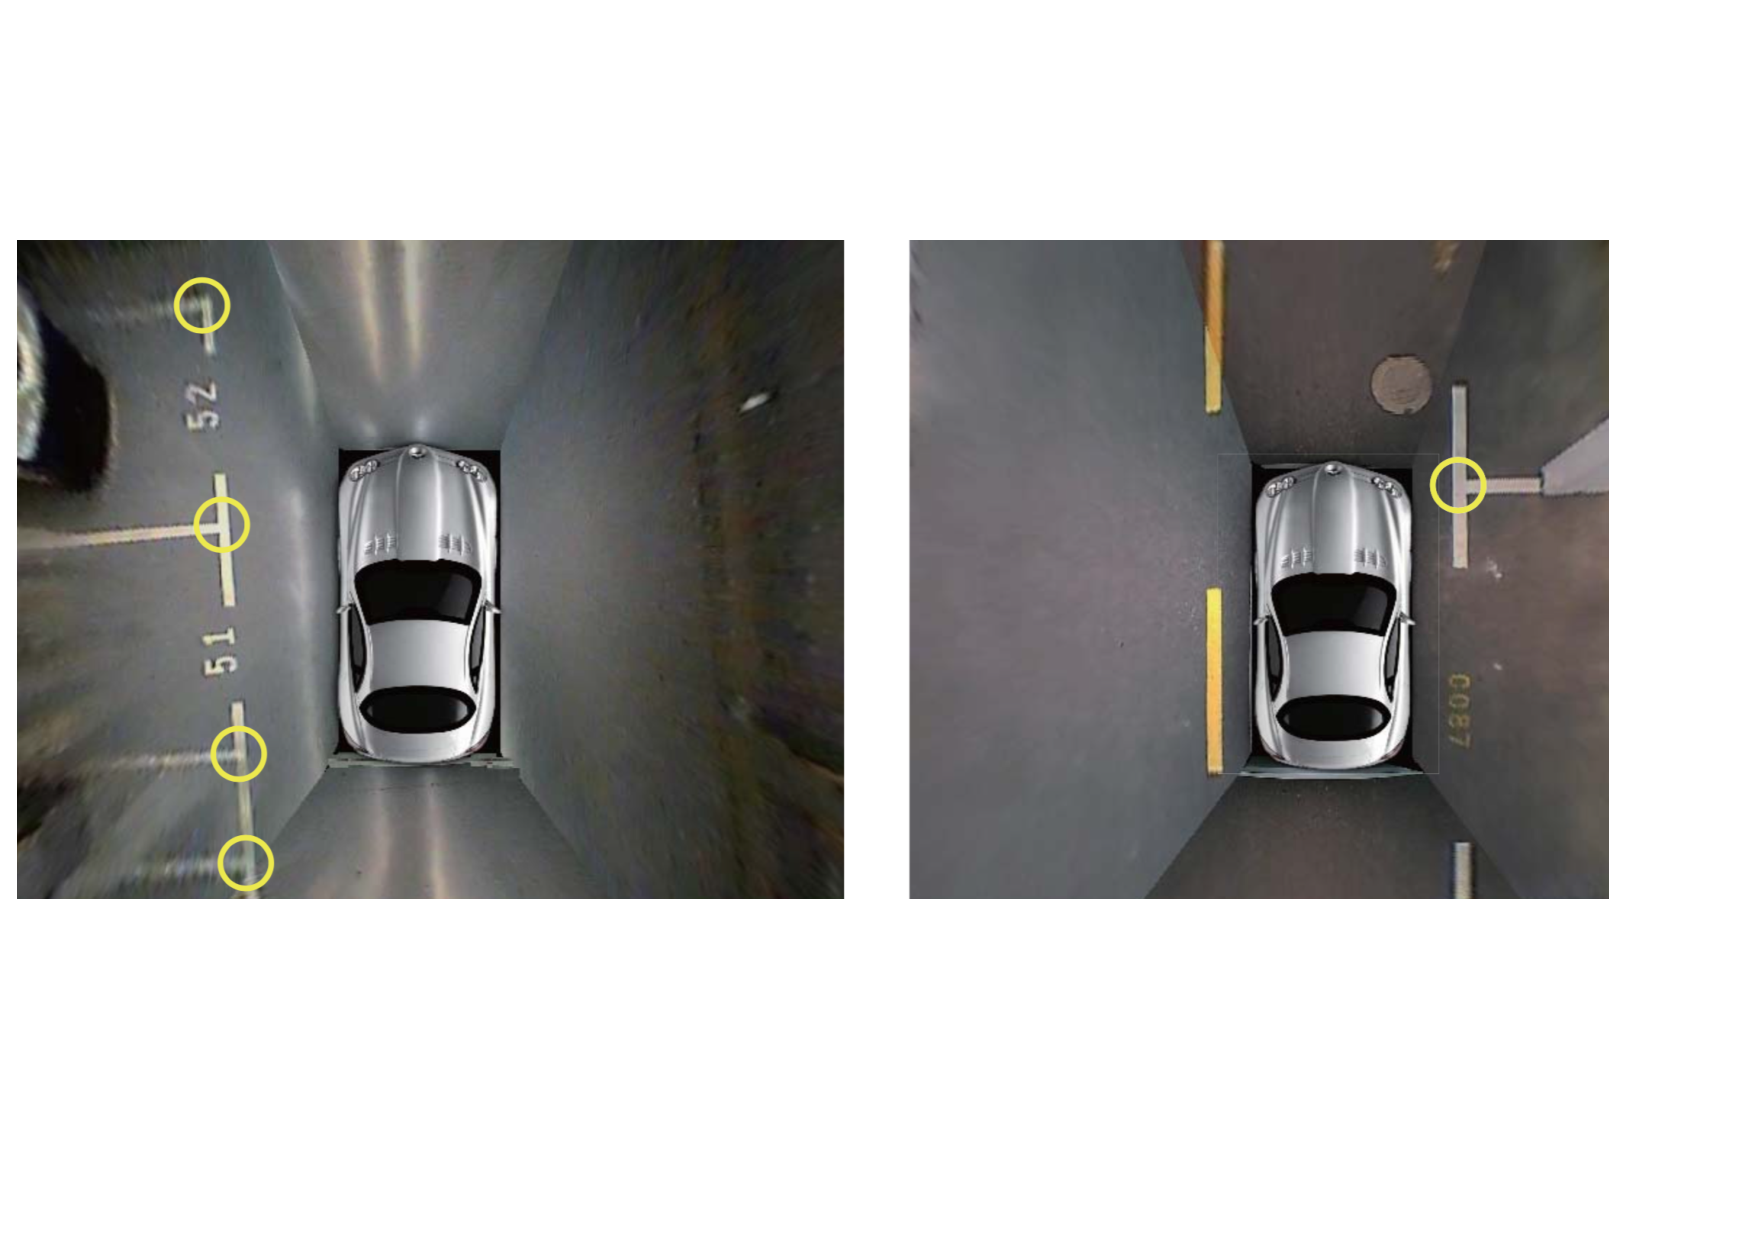
\includegraphics[width=12cm, height=5cm]{images/markingPoint1.pdf} \\
         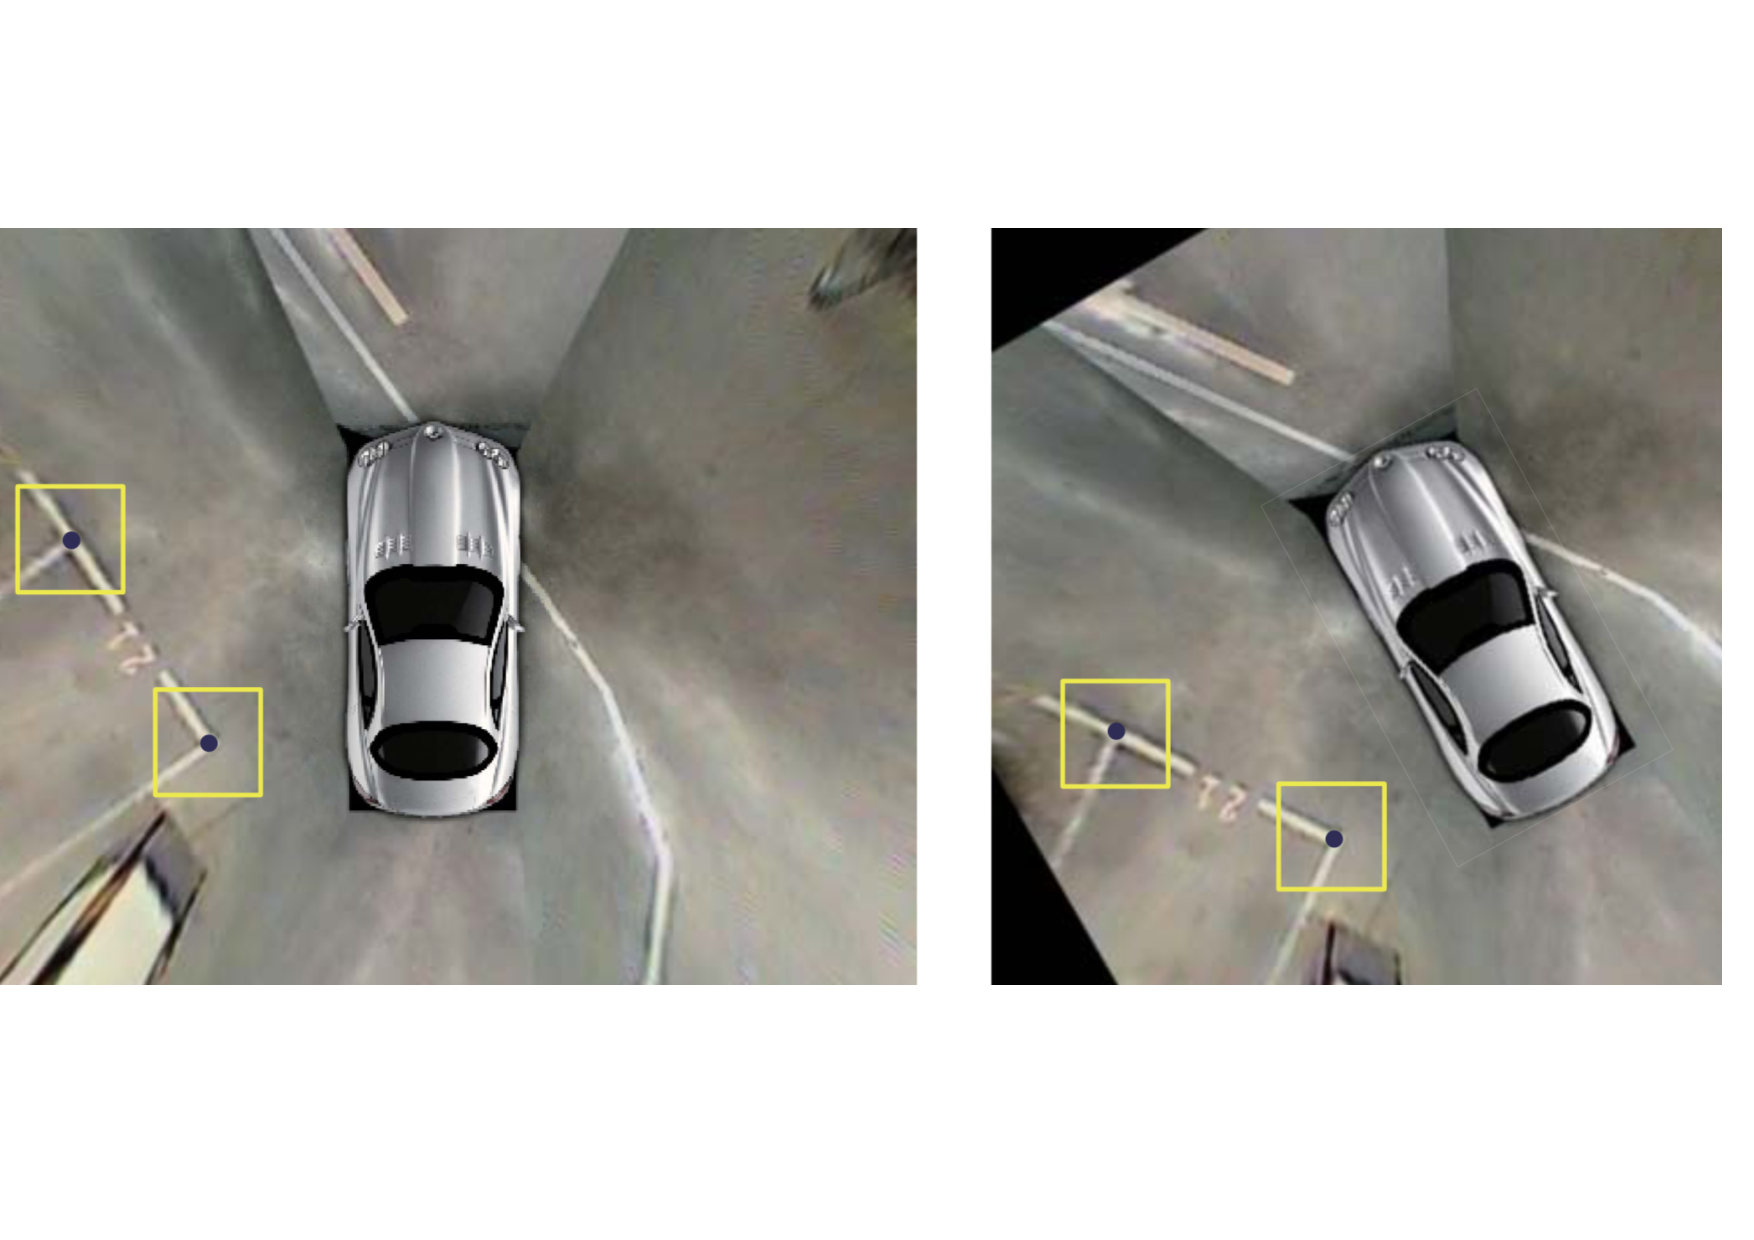
\includegraphics[width=12cm, height=5cm]{images/markingPoint2.pdf}
    \end{tabular}
    \caption{Marking points to define parking lots \cite{markingPointJournal}}
    \label{fig:markingPoint}
\end{figure}
Here surrounded view images of different car direction are used to detect marking points where a binary classifier applied to all local images in data base for detection. Then parking places are detected from these marking points. The approach is to take every two cross points of two parking segments and according to their lengths by applying a pattern called Gaussian line temple, parking lots will be detected. They completed their algorithm in \cite{markingPointJournal} by using \acrshort{nn} and DCNN based Networks and also a bigger data base of surrounding view images. For training process \acrshort{yolo}2 method base on DCNN has been used and during training process, position of all marking points in dataset(surrounding images) has to be learned. There are number of rotations for each image in database. After detection of marking point, in the next step, a pattern classifier for marking points will be used to define which points are in the same class and which two cross points make valid entrance line for parking. Finally in the last step, depth of the parking slot will be measured and find which of the points sets in the last step, make a rectangular which is a parking lot. Although This method is really perfect and it precisely defines parking places, it does not clarify whether the parking place is empty or occupied. For parking occupancy detection we could refer to Bayes classifier methods and Region Growing Algorithm. \cite{visual-parking-slot} used Bayes classifier for feature extraction and classification of parking slots and available parking lots were detected based on this features. In order to figure out whether a parking lot contains a car, region growing algorithm has been used. The approach is to examine pixels of parking lot images as it calculate each pixel of the image and in each step examines the neighboring pixels of initial points and determines whether the neighbors are similar to the initial ones. When the neighboring pixels are different from the last ones, it means that they contains vehicles. \cite{empty-parking-vision} proposed a method to distinguish empty parking places from occupied ones by segmentation of parking area into blocks using calibration. The approach is to covert image into gray-scale blocks and in each block white color refers to car and if the block is black, it means that it does not contain a car and it's a free parking lot. Threshold value is calculated in every block to determine if the block contains white color(car) or that is empty. \cite{US-visionbased} is another method to determine occupied parking places based on 3-layer Bayesian hierarchical detection framework or BHDF. Based on the geometric structure of parking slots divides them to car occlusions and environment occlusions. Prior knowledge to the network is required for this segmentation and training step is based on the labeling of the vehicles so when the method could not find vehicle in the image, it would be classified as environment occlusion. \cite{histogramEOH} also represents a way of parking space detection based on edge orientation histogram (EOH) density. The novelty of this approach is that it could handle object detection in dynamic light effects and even in dark images and night scenes which was not possible in last methods. They claim that this method could work with low quality of camera and in different light setting in parking area. To make this algorithm work in different light setting, they used dynamic mixing of multiple features as these multiple features make algorithm strong enough to detect objects in variant lights. 

\section{Path-Planning and Motion-Generation}
After determination of empty parking lots, it's time to maneuver. Various algorithms for generation of path motion and parking maneuver has been proposed during last decade. As it has been explained in \ref{chapter:introduction} there are two types of path-planning. Here are some examples from both methods:
\subsection{Fuzzy Logic Control}
In this method, human driving experience are gathered to create a database which is in the form of IF-THEN rules. These rules shows the steps to a robot or a selfless car \cite{novel-CLMR}. This database needs to be trained in advance and the goal is to control the vehicle  to the desired position by using these rules on database. Fuzzy system should select suitable movement at each time from the knowledge database according to its internal states. \cite{fuzzy} Uses fuzzy parking control method to control the steering angle of a \acrfull{clmr}. They proposed different methods for forward and backward maneuver and also applied their algorithm for both garage and parallel parking so in total 4 movement methods have been defined. Backward and forward Fuzzy Garage Parking Control(FGPC) and 2 methods for Backward and forward Fuzzy Parallel Parking Control(FPPC). Real-time image processing was used to define the next motion. Image information were used to define next movement and end position. Color detection method was used to calculate the end position. A host computer which connected to the robot were capturing the working environment via the vision system and calculation of the posture of \acrshort{clmr} by analyzing image information and sends commands which contains the next movements to the robot/CLMR via wireless radio modem. We can refer to \cite{machine-learning-parking} as another example. Here the idea was based on the decomposition of a parking maneuver into sub-maneuvers that could be realized in an open loop control so the main challenge was the transition between these sub-maneuvers which could be done by machine learning classifiers. RF-kernel was used as a learning classifier and General Radial Basis Function (GRBF) classifier was used to find the similarities based on the template. Classifiers were trained to find the detection points where transition from one sub maneuver to to the next one is required. So the idea was to find the best position of the vehicle based on machine learning. Here machine algorithms helps to find features through images and detect vehicle position then determine whether the posture of vehicle is good respects to the map of the parking area or decide if the maneuver should be done.
\subsection{Reference Trajectory }
This method is  based on a reference path as the path depends on the environment model as well as the vehicle model like its speed, steering and etc. 
%As the early works in this area, we could refer to Van Brussel et al.\cite{} as they developed their path algorithm based on combining  motion-primitives-lines and circles.
Igor Paromtchik and his colleague from INRIA institute \cite{parkingManeuver} developed a smooth motion algorithm which was applied to LIGIER electric vehicle of French company. They presented an iterative algorithm which used a combination of feedback and planning approach. Maneuver consisted of N-iterative motions aimed at lateral displacement of the vehicle. The idea was to control the vehicle maneuver based on its velocity and steering angle. They used 14 ultrasonic sensors for the range measurements and getting information from the environment. K. Jiang et al. in \cite{twoCircles}, believed that algorithm represented in \cite{parkingManeuver} was not considering possible collision and longitudinal boundary during maneuver. So they proposed a new algorithm by defining some constraints for parking maneuver i,e. they defined forbidden area for movement in parking lot as we could see in fig \ref{fig:forbiddenArea}.
\begin{figure}
    \centering
    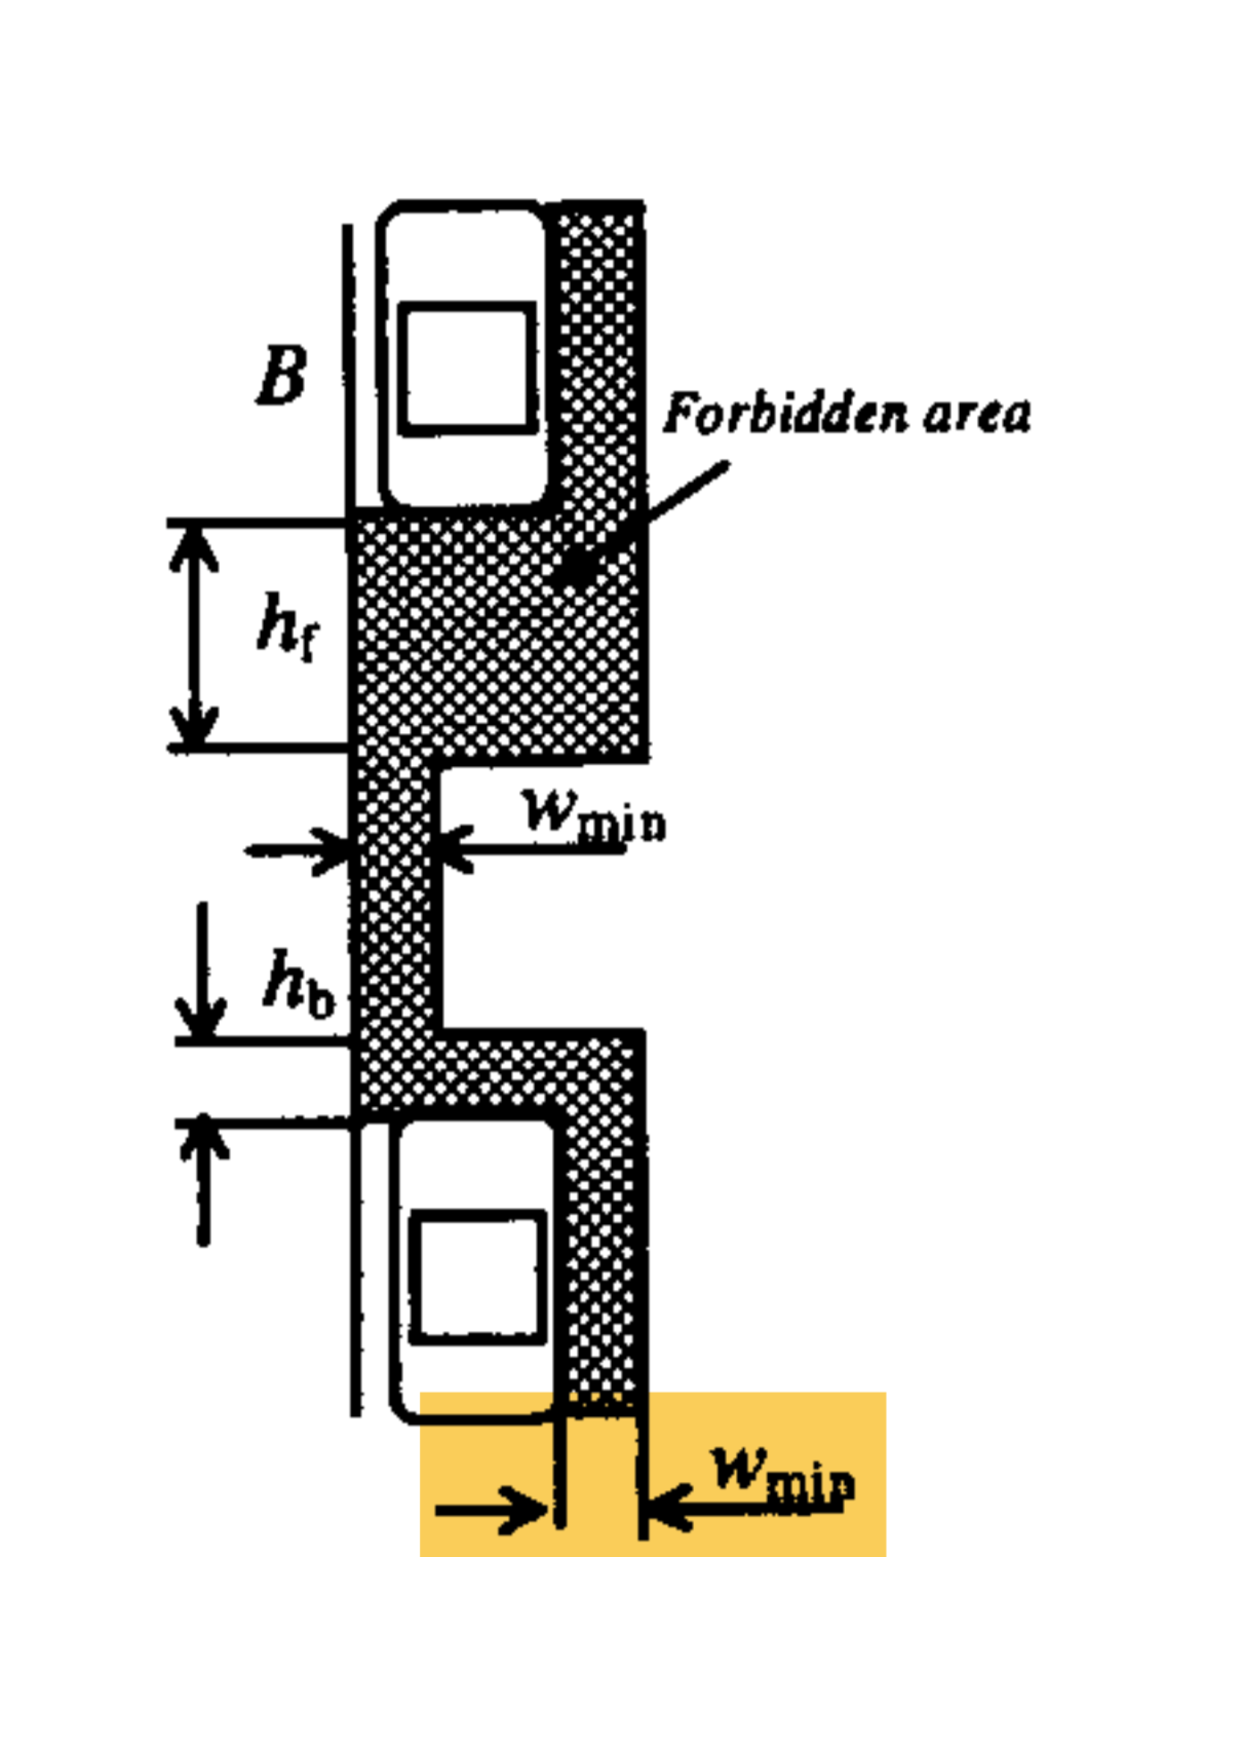
\includegraphics[width=9cm, height=7cm]{images/forbiddenArea.pdf}
    \caption{Forbidden area in parallel parking maneuver \cite{twoCircles}}
    \label{fig:forbiddenArea}
\end{figure}
Motion path was formed by two circles(or 2 arcs). One of the circle movement is clockwise and the other one is in opposite direction for controlling forward and backward movements as they are in opposite direction. Fig \ref{fig:2CirclePath} illustrates the path.
\begin{figure}
    \centering
    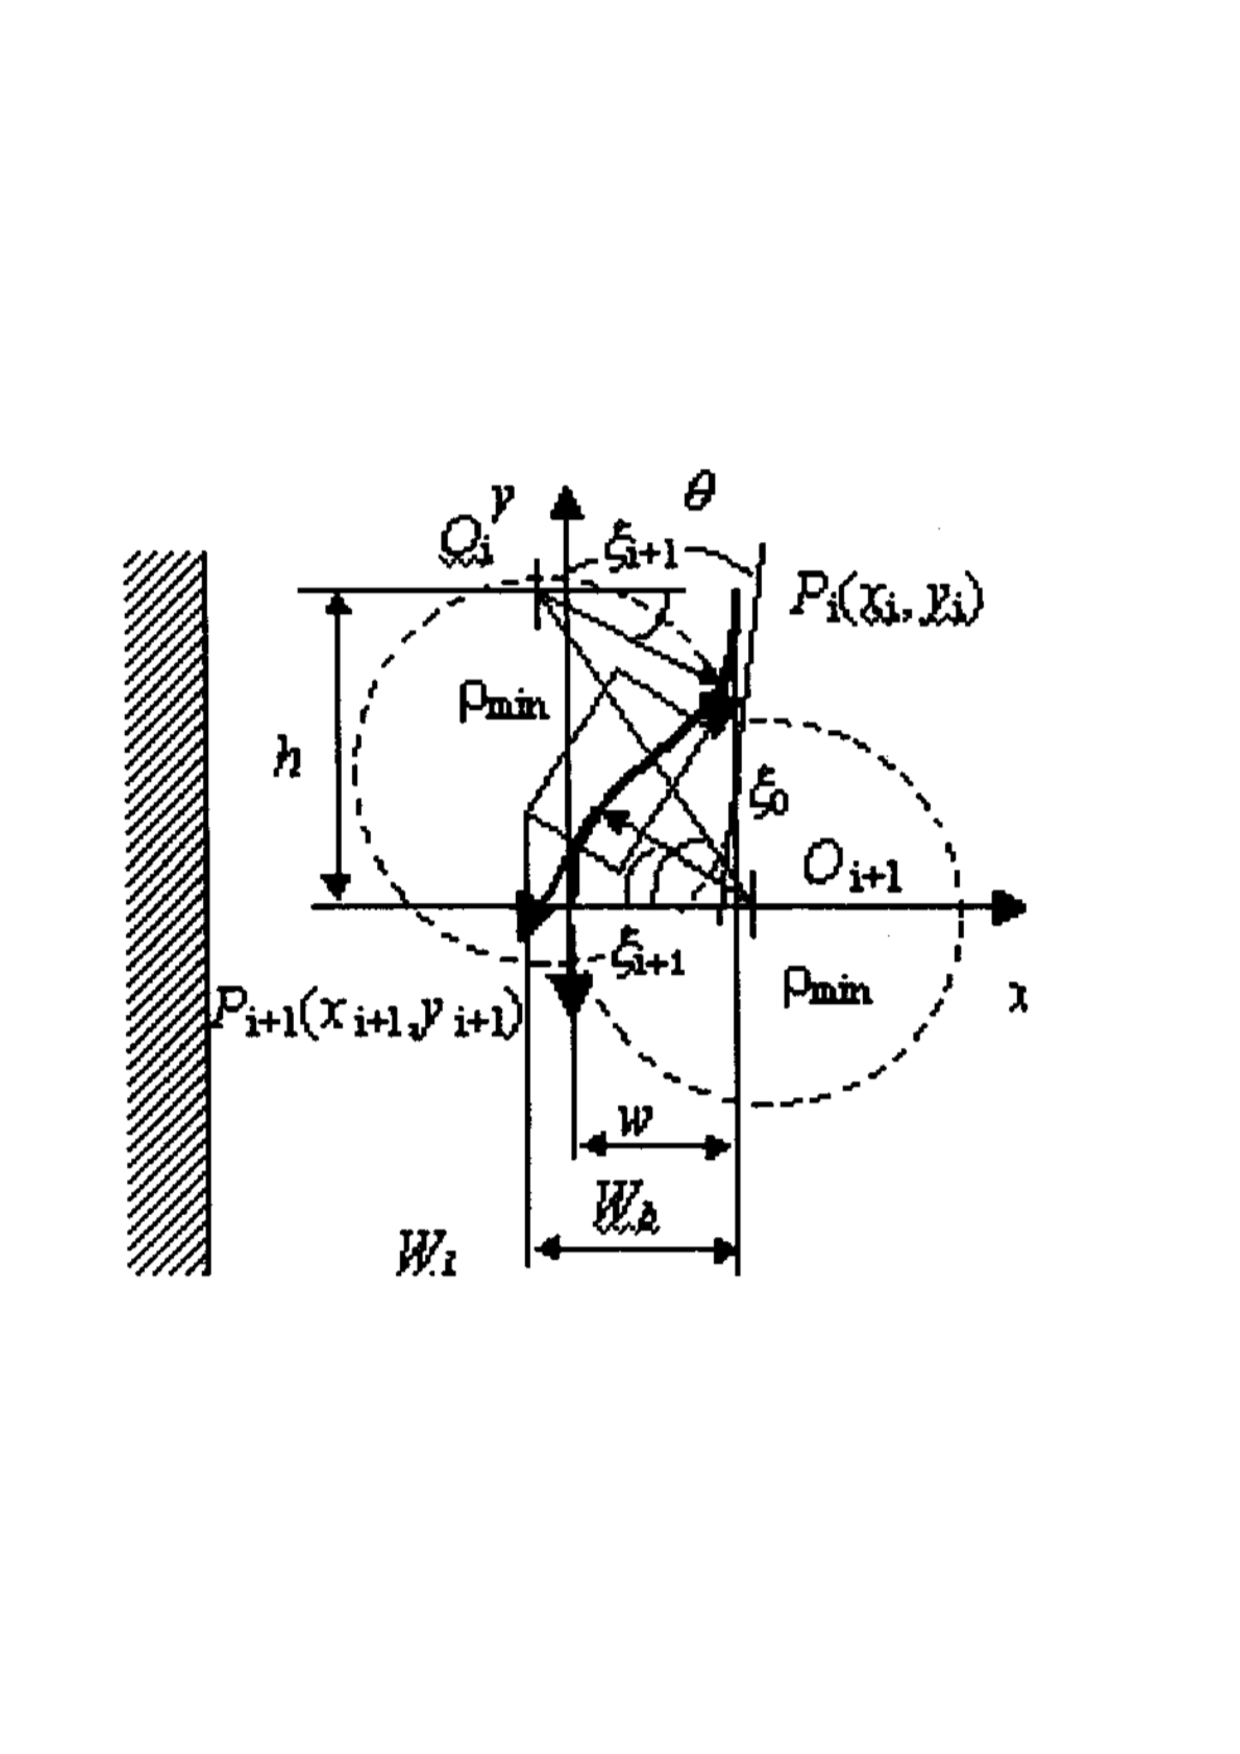
\includegraphics[width=9cm, height=7cm]{images/2circlePath.pdf}
    \caption{Motion-path formed by two circular arcs\cite{twoCircles}}
    \label{fig:2CirclePath}
\end{figure}
This algorithm planned a path for robot or \acrshort{clmr} outside of the forbidden area. They claims that their algorithm could also work in a small parking spaces. However, the last method was applied on a real car and that is still used for LIGIER autonomous vehicles and this one was just implemented on a \acrshort{clmr}. \cite{novel-CLMR} presents another example of reference path method which is only for vertical parking lots.
